\documentclass[12pt]{report}
\usepackage[thinc]{esdiff} % for typesettign derivatives
\usepackage{amsthm} % provides an enhanced version of LaTex's \newtheorem command
\usepackage{mdframed} % framed environments that can split at page boundaries
\usepackage{enumitem} % bulletin points or other means of listing things
\usepackage{amssymb} % for AMS symbols
\usepackage{amsmath} % so as to use align
\usepackage{latexsym} % so as to use symbols like \leadsto
\usepackage{mathrsfs} % for using mathscr for char like operators
\usepackage{commath} % for using norm symbol
\usepackage{authblk} % for writing affiliations
\usepackage{graphicx} % for importing images
\graphicspath{{./images/}} % for the path to images, also always put label behind captions
\usepackage{textcomp} % for using degree symbol
\usepackage{hyperref} % for clickable link in the pdf & customizable reference text
\usepackage[all]{hypcap} % for clickable link to images instead of caption
\usepackage[margin=1in]{geometry} % default is 1.5in
% \usepackage[left=0.4in, right=0.4in, top=0.8in, bottom=0.8in]{geometry}
\usepackage[title]{appendix} % for attaching appendix
\allowdisplaybreaks % allow page breaking in display maths, like align
% allow for more advanced table layout
\usepackage{booktabs}
\usepackage{multirow}
\usepackage{siunitx}

\theoremstyle{definition}
\mdfdefinestyle{defEnv}{%
  hidealllines=false,
  nobreak=true,
  innertopmargin=-1ex,
}

% The following is for writing block of code
\usepackage{listings}
\usepackage{color}

\definecolor{dkgreen}{rgb}{0,0.6,0}
\definecolor{gray}{rgb}{0.5,0.5,0.5}
\definecolor{mauve}{rgb}{0.58,0,0.82}

% Use the following to change code language and related settings
\lstset{frame=tb,
  language=Python,
  aboveskip=3mm,
  belowskip=3mm,
  showstringspaces=false,
  columns=flexible,
  basicstyle={\small\ttfamily},
  numbers=none,
  numberstyle=\tiny\color{gray},
  keywordstyle=\color{blue},
  commentstyle=\color{dkgreen},
  stringstyle=\color{mauve},
  breaklines=true,
  breakatwhitespace=true,
  tabsize=3
}

\pagestyle{headings}
\author{Lectured by Martin Rasmussen}
\title{DE condensed notes}
\affil{Typed by Aris Zhu Yi Qing}
\begin{document}
\maketitle
\tableofcontents

\chapter{Introduction}

\section{Ordinary Differential Equation (ODE) and Initial Value Problems (IVP)}

\newmdtheoremenv[style=defEnv]{theorem}{Definition}
\begin{theorem}
    Consider $d\in\mathbb{N}$, an open set $D \subset
    \mathbb{R}\times\mathbb{R}^{d}$, and a function
    $f:D\rightarrow\mathbb{R}^{d}$. An equation of the form
    \[
        \dot{x} = f(t,x)
    \]
    is called a \textbf{$d$-dimensional (first-order) ODE}.
    A differentiable function $\lambda:I\rightarrow\mathbb{R}^{d}$
    on an interval $I\subset \mathbb{R}$ is called a solution to the
    above differential equation if $(t,\lambda(t))\in D$ and\[
        \dot{\lambda}(t)=f(t,\lambda(t)) \quad \forall t\in I.
    \]
    Specially, an ODE is \textbf{autonomous} if the equations is of the form
    \[
        \dot{x} = f(x),
    \]
    where $f:D\rightarrow\mathbb{R}^{d}$ for some open set
    $D\subset\mathbb{R}^{d}$.
\end{theorem}

\newmdtheoremenv[style=defEnv]{constant solutions to autonomous ODE}[theorem]{Proposition}
\begin{constant solutions to autonomous ODE}\label{constant solutions to autonomous ODE}
    Consider an open set $D\subset\mathbb{R}^{d}$ and a function
    $f:D\rightarrow\mathbb{R}^{d}$, and consider the autonomous ODE
    \[
        \dot{x} = f(x),
    \]
    then $\exists \lambda:\mathbb{R}\rightarrow\mathbb{R}^{d}, a\in\mathbb{R}^{d}$
    s.t. $\forall t\in\mathbb{R},\lambda(t)=a$ iff $f(a)=0$.
\end{constant solutions to autonomous ODE}

\newmdtheoremenv[style=defEnv]{IVP}[theorem]{Definition}
\begin{IVP}
    Consider $d\in\mathbb{N}$,
    an open set $D\subset \mathbb{R}\times\mathbb{R}^{d}$,
    and a function $f:D\rightarrow\mathbb{R}^{d}$.
    The combination of the ODE\[
        \dot{x}=f(t,x)
    \]with an initial condition of the form\[
        x(t_0)=x_0
    \]
    where $(t_0,x_0)\in D$, is called an \textbf{Initial Value Problem (IVP)}.
\end{IVP}

\section{Examples}

The ODE ideally satisfies the following three conditions:
\begin{enumerate}[label = (\roman*)]
    \item A solution \textbf{exists} for every IVP.
    \item The solution to each IVP is \textbf{unique}.
    \item The solution to each IVP \textbf{exists globally},
        i.e.\ can be defined on $I=\mathbb{R}$.
\end{enumerate} 
Now we look at examples which not all of the aforementioned properties are
satisfied.

\newtheorem{No solution to an IVP}[theorem]{Example}
\begin{No solution to an IVP}
    Consider the 1-dimensional IVP
    \[
        \dot{x}=f(x)=
        \begin{cases}
            1 & x<0 \\
            -1 & x\ge 0
        \end{cases},\quad x(0)=0
    \]
    which has a discontinuous right hand side. 
    Since $x(0)=0$, we have $\dot{x}(0)=-1$.
    Also, $\exists \tau>0$ s.t. $\forall 0<t<\tau$, $x(t)<0$ and $\dot{x}=1$.
    This contradicts with MVT, that
    \[
        \exists 0<\mu<\frac{\tau}{2} \text{ s.t. }
        \dot{x}(\mu)=\frac{x(\frac{\tau}{2})-x(0)}{\frac{\tau}{2}}.
    \]
\end{No solution to an IVP}

\newtheorem{Many solutions to an IVP}[theorem]{Example}
\begin{Many solutions to an IVP}
    Consider the 1-dimensional IVP
    \[
        \dot{x}=\sqrt{|x|}, \quad x(0)=0.
    \]
    Since $f(0)=0$, Proposition~\ref{constant solutions to autonomous ODE}
    implies that there exists a constant solution with value 0.
    In addition, for any $b\ge 0$, the function
    $\lambda_b:\mathbb{R}\rightarrow\mathbb{R}$,
    \[
        \lambda_b(t)=
        \begin{cases}
            0, & t\le b \\
            \frac{1}{4}(t-b)^{2}, & t>b
        \end{cases} 
    \]
    is a solution to this IVP.
\end{Many solutions to an IVP}

\newtheorem{Solutions do not need to exist for all times}[theorem]{Example}
\begin{Solutions do not need to exist for all times}
    Consider the IVP
    \[
        \dot{x}=tx^{2}, \quad x(t_0)=x_0,
    \]
    where $x_0\neq 0$. Using the procedure of \textbf{separation of variables},
    i.e.\
    \[
        \frac{\mathrm{d}x}{\mathrm{d}t}=g(t)h(x) \Rightarrow
        \frac{\mathrm{x}}{h(x)}=g(t)\mathrm{d}t,\; x(t_0)=x_0
    \]
    \[
        \Rightarrow \int_{x_0}^{x} \frac{1}{h(y)}\mathrm{d}y
        = \int_{t_0}^{t} g(s)\mathrm{d}s
    \]
    and solving the above equation w.r.t. $x$ to give the solution,
    we get
    \[
        \frac{\mathrm{d}x}{x^{2}}=t\mathrm{d}t\Rightarrow
        \frac{1}{x_0}-\frac{1}{x}=\frac{t^{2}}{2}-\frac{t_0^{2}}{2},
        \;x(t_0)=x_0
    \]
    \[
        \Rightarrow x=\frac{2x_0}{2+x_0(t_0^{2}-t^{2})}.
    \]
    We can then see that all solutions with $x_0>0$ are defined on the bounded
    subinterval $(-\sqrt{2}, \sqrt{2})\subset\mathbb{R}$ when $t_0=0$ and $x_0=1$.
\end{Solutions do not need to exist for all times}

\section{Visualization}

\subsection{Solution Portrait}

We consider a function
$f:D\subset\mathbb{R}\times\mathbb{R}^{d}\rightarrow\mathbb{R}^{d}$
and the corresponding ODE
\[
    \dot{x}=f(t,x),
\]
a solution to this equation is a differentiable function
$\lambda:I\rightarrow\mathbb{R}^{d}$ fulfilling
$\dot{\lambda}(t)=f(t,\lambda(t))$ on the interval $I$.
Then the graph of this solution, given by the so-called 
\textbf{solution curve}
\[
    G(\lambda)=\left\{(t,\lambda(t)):t\in I\right\}
    \subset\mathbb{R}\times\mathbb{R}^{d},
\]
is a differentiable curve. The derivative of this curve in the point
$t_0\in I$ is given by 
$\frac{\mathrm{d}}{\mathrm{d}t}(t,\lambda(t))|_{t=t_0}=(1,\dot{\lambda}(t_0)
= (1, f(t_0, \lambda(t_0)))$.
This implies that in particular that the vector field
\[
    (t,x)\mapsto(1,f(t,x)),
\]
defined on $D$ is crucial for the shape of the solution curves.

\medskip
\noindent A \textbf{solution portrait} is given by a visualization of several solution
curves, in the $(t,x)$-space, the so-called \textbf{extended phase space}.
The $x$-space is normally called the \textbf{phase space}.

\subsection{Phase portrait}

\newmdtheoremenv[style=defEnv]{translation invariance}[theorem]{Proposition}
\begin{translation invariance}
    Let $\lambda:I\rightarrow\mathbb{R}^{d}$ be a solution to the
    autonomous differential equation
    \[
        \dot{x}=f(x).
    \]
    Then $\forall \tau\in\mathbb{R}$, the function
    $\mu:\tilde{I}\rightarrow\mathbb{R}^{d}$, where
    $\tilde{I}:=\left\{t\in\mathbb{R}:t+\tau\in I\right\}$ and
    \[
        \mu(t):=\lambda(t+\tau) \quad \forall t\in\tilde{I},
    \]
    is also a solution to this differential equation.
\end{translation invariance}

\begin{proof}
    Since $\lambda$ is a solution, we have $\dot{\lambda}(t)=f(\lambda(t))$
    for $t\in I$. The chain rule implies that $\forall t\in\tilde{I}$,
    $\dot{\mu}(t)=\dot{\lambda}(t+\tau)$, and we get that $\forall t\in\tilde{I}$,
    \[
        \dot{\mu}(t)=\dot{\lambda}(t+\tau)=f(\lambda(t+\tau))=f(\mu(t))
    \]
\end{proof} 

\begin{figure}[h]
  	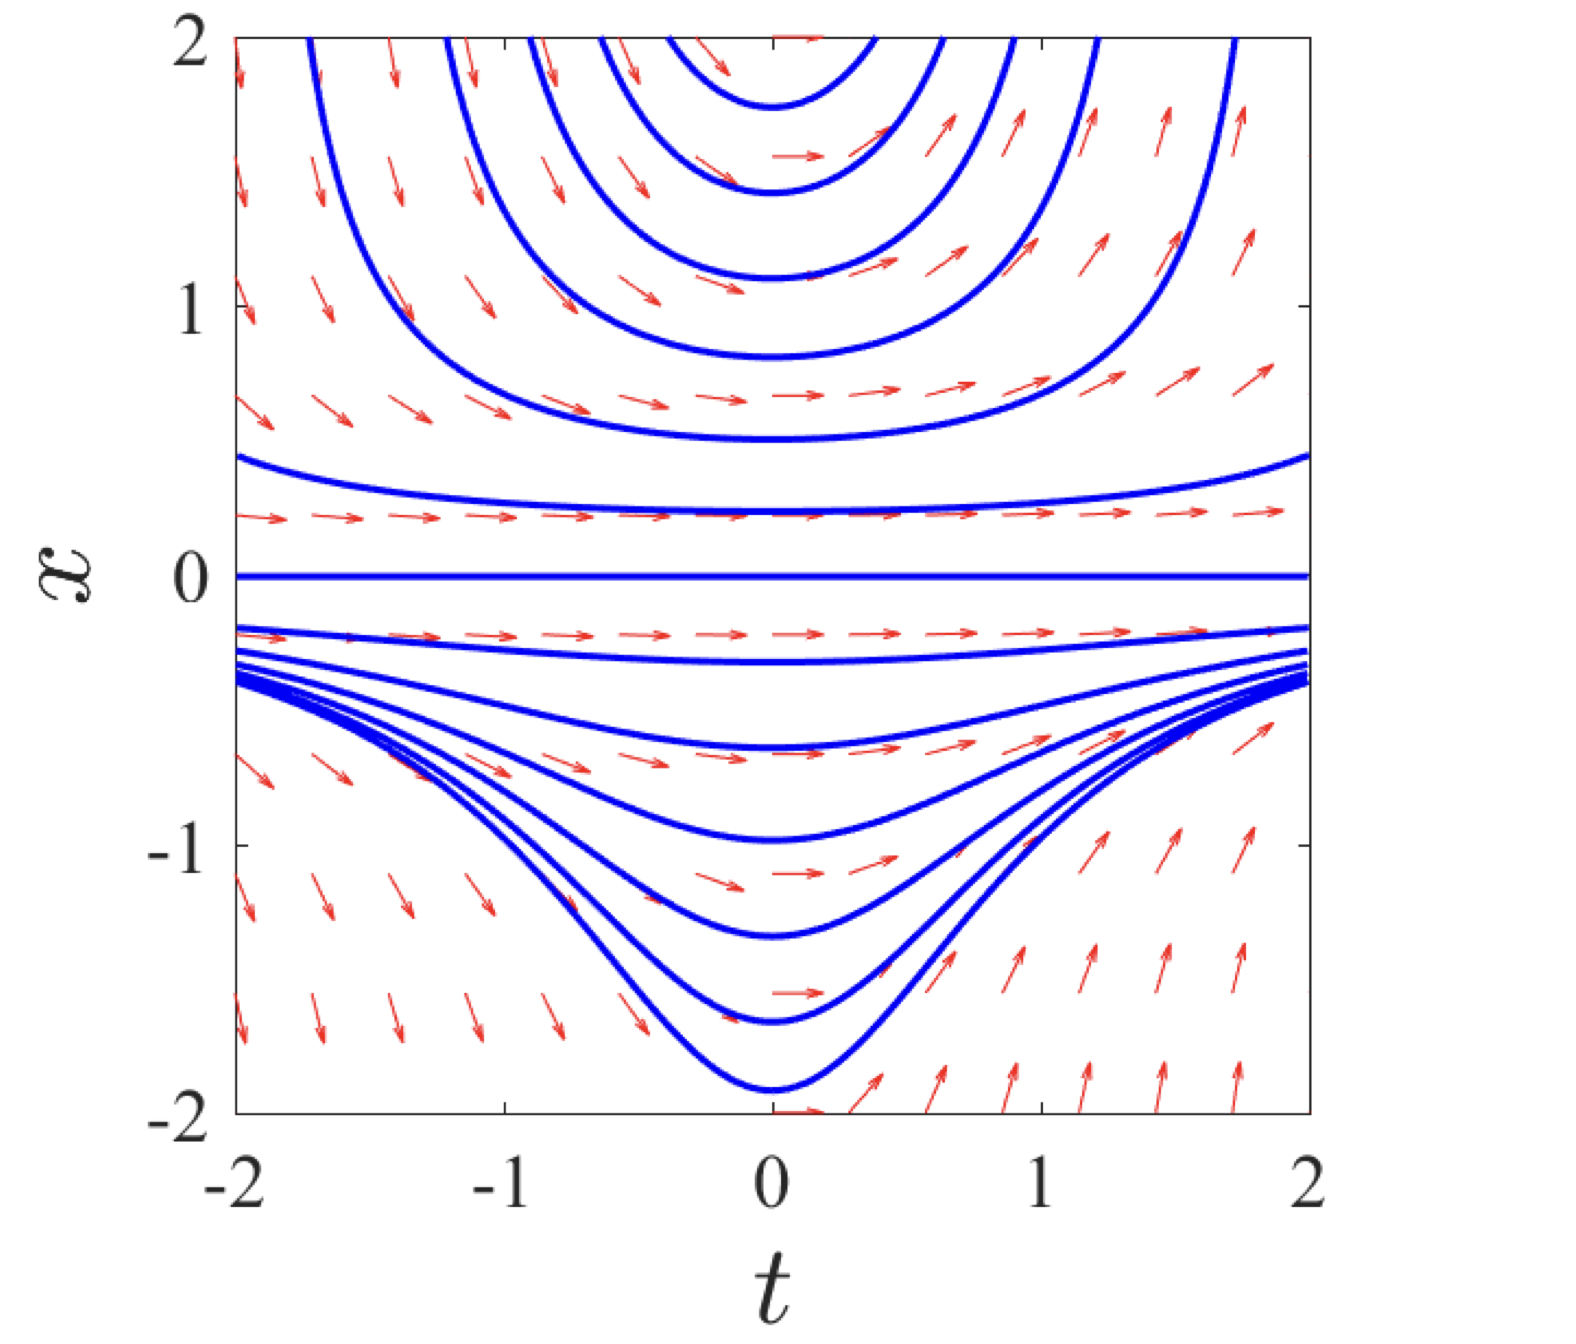
\includegraphics[scale=0.2]{./images/phase_portrait1.jpeg}
  	\centering
    \caption{phase portrait for $\dot{x}=tx^{2}$}
\end{figure}

\begin{figure}
  	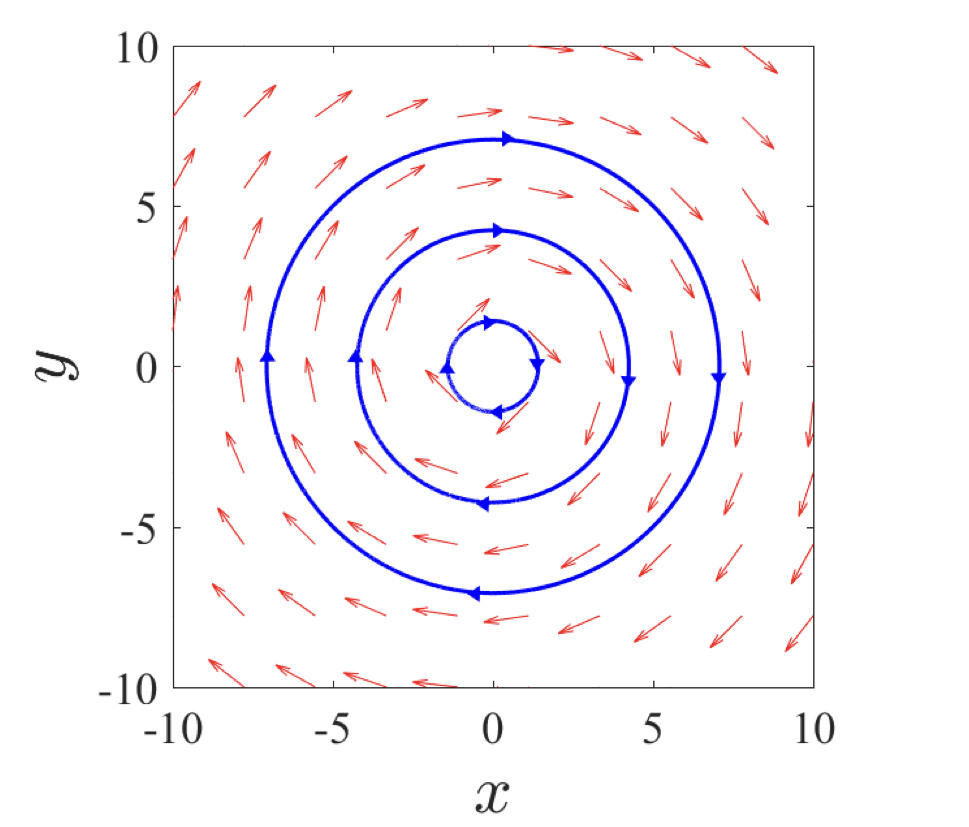
\includegraphics[scale=0.4]{./images/phase_portrait2.jpeg}
  	\centering
    \caption{phase portrait for $\ddot{x}=-x$}
\end{figure}


\chapter{Existence and Uniqueness}

\section{Picard iterates}

\newmdtheoremenv[style=defEnv]{reformulation as integral equation}[theorem]{Proposition}
\begin{reformulation as integral equation}
    Consider the IVP
    \[
        \dot{x}=f(t,x), \quad x(t_0)=x_0,
    \]
    where $f:D\subset\mathbb{R}\times\mathbb{R}^{d}\rightarrow\mathbb{R}^{d}$
    is continuous and $(t_0, x_0)\in D$, and let 
    $\lambda:I\rightarrow\mathbb{R}^{d}$ be a function on an interval $I$
    s.t. $t_0\in I$ and $\left\{(t,\lambda(t)):t\in I\right\}\subset D$.
    Then the following two statements are equivalent.
    \begin{enumerate}[label = (\roman*)]
        \item $\lambda$ solves the IVP, i.e.\
            \[
                \dot{\lambda}(t)=f(t, \lambda(t)) \quad\forall t\in I,
                \text{ and } \lambda(t_0)=x_0.
            \]
        \item $\lambda$ is continuous, and we have
            \[
                \lambda(t)=x_0+\int_{t_0}^{t}f(s,\lambda(s))\mathrm{d}s
                \quad\forall t\in I.
            \]
    \end{enumerate} 
\end{reformulation as integral equation}

\newmdtheoremenv[style=defEnv]{Picard iterates}[theorem]{Definition}
\begin{Picard iterates}
    Consider the IVP, and choose an interval $J$ that contains $t_0$.
    We define an initial function
    \[
        \lambda_0(t)\equiv x_0\quad\forall t\in J,
    \]
    and inductively, the Picard iterates
    \[
        \lambda_{n+1}(t):=x_0+\int_{t_0}^{t}f(s,\lambda_n(s))\mathrm{d}s
        \quad\forall t\in J \text{ and } n\in\mathbb{N}_0.
    \]
\end{Picard iterates}

\newtheorem{picard iterates example}[theorem]{Example}
\begin{picard iterates example}
    We would like to compute the Picard iterates for the IVP
    \[
        \dot{x}=ax, \quad x(t_{0})=x_0,
    \]
    where $a\in\mathbb{R}$ is fixed. The first three iterates are
    \begin{align*}
        \lambda_0(t) & = x_0, \\
        \lambda_1(t) & = x_0 + \int_{t_0}^{t} ax_0\mathrm{d}s
        = x_0(1+a(t-t_0)), \\
        \lambda_2(t) & =x_0+\int_{t_0}^{t}ax_0(1+a(s-t_0))\mathrm{d}s
        = x_0(1+a(t-t_0)+\frac{1}{2}a^{2}(t-t_0)^{2}). \\
        \vdots
    \end{align*}
\end{picard iterates example}

\section{Lipschitz continuity}

\newmdtheoremenv[style=defEnv]{normed vector space}[theorem]{Definition}
\begin{normed vector space}
    A \textbf{norm} on a vector space $V$ over the reals is a map
    $\norm{\cdot}:V\rightarrow\mathbb{R}_0^{+}$ s.t.
    \begin{enumerate}[label = (\roman*)]
        \item $\norm{x}=0 \iff x=0$. 
                (positive definiteness)
        \item $\norm{ax}=|a| \norm{x} \;\forall a\in\mathbb{R}$ and $x\in V$. 
            (absolute homogeneity)
        \item $\norm{x+y}\le\norm{x}+\norm{y} \;\forall x,y\in V$. 
            (triangle inequality)
    \end{enumerate} 
    A vector space with norm is called a \textbf{normed vector space}.
\end{normed vector space}

\newmdtheoremenv[style=defEnv]{continuous and lipschitz continuous functions}[theorem]{Definition}
\begin{continuous and lipschitz continuous functions}
    Let $X$ be a subset of a normed vector space $(V, \norm{\cdot}_V)$ and $Y$
    be a subset of a normed vector space $(W, \norm{\cdot}_W)$.
    Then a function $f:X\rightarrow Y$ is called
    \begin{enumerate}[label = (\roman*)]
        \item \textbf{continuous} if $\forall x\in X, \epsilon > 0$,
            $\exists \delta>0$ s.t.
            \[
                \norm{x-\overline{x}}_V<\delta \Longrightarrow
                \norm{f(x)-f(\overline{x})}_W < \epsilon.
            \]
        \item \textbf{Lipschitz continuous} if $\exists K>0$ s.t.
            \[
                \norm{f(x)-f(\overline{x})}_W\le K\norm{x-\overline{x}}_V
                \quad\forall x,\overline{x}\in X.
            \]
            The constant $K$ is called a \textbf{Lipschitz constant}.
    \end{enumerate} 
\end{continuous and lipschitz continuous functions}

\subsection{Lipschitz continuity and the mean value theorem (MVT)}

Recall that the mean value theorem says that for any $x,y\in I$,
$\exists \xi$ between $x$ and $y$ s.t.
\[
    f(x)-f(y)=f'(\xi)(x-y).
\]
This implies that
\[
    \left|f(x)-f(y)\right|=|f'(\xi)||x-y|,
\]
and it is clear that if the derivative $f'$ is bounded on the interval $I$,
then $f$ is Lipschitz continuous.

\subsection{Lipschitz continuity and the mean value inequality}

\newmdtheoremenv[style=defEnv]{operator norm of a matrix}[theorem]{Definition}
\begin{operator norm of a matrix}
    For a given matrix $A\in\mathbb{R}^{m\times n}$,
    the \textbf{operator norm} of $A$ is defined by
    \[
        \norm{A}:= \underset{x\in\mathbb{R}^{n}\backslash\{0\}}{\sup}
        \frac{\norm{Ax}}{\norm{x}},
    \]
    which can be calculated by finding the square root of the largest
    eigenvalue of $A^{T}A$.
\end{operator norm of a matrix}

\newmdtheoremenv[style=defEnv]{mean value inequality}[theorem]
{(Mean Value Inequality) Theorem}
\begin{mean value inequality}
    Consider an open set $D\subset \mathbb{R}^{n}$, and let 
    $f:D\rightarrow\mathbb{R}^{m}$ be continuously differentiable.
    Then $\forall x,y\in D$ with $[x,y]\subset D$, $\exists \xi\in[x,y]$ s.t.
    \[
        \norm{f(x)-f(y)}\le\norm{f'(\xi)}\norm{x-y},
    \]
    where for any $x,y\in\mathbb{R}^{n}$,
    $[x,y]:=\{\alpha x+(1-\alpha)y\in\mathbb{R}^{n}:\alpha\in[0,1]\}$.
\end{mean value inequality}

\newmdtheoremenv[style=defEnv]{triangle-like inequality for integrals}[theorem]{Lemma}
\begin{triangle-like inequality for integrals}
    Let $I\subset \mathbb{R}$ be an interval and $f:I\rightarrow\mathbb{R}^{m}$
    be a continuous function. Then
    \[
        \norm{\int_{t_0}^{t}f(s)\mathrm{d}s}\le\left|\int_{t_0}^{t}
        \norm{f(s)}\mathrm{d}s\right|
        \quad\forall t, t_0\in I.
    \]
\end{triangle-like inequality for integrals}

\newmdtheoremenv[style=defEnv]{Lipschitz continuity and the mean value inequality}[theorem]{Corollary}
\begin{Lipschitz continuity and the mean value inequality}
    Let $U\subset\mathbb{R}^{n}$ be open and $f:U\rightarrow\mathbb{R}^{m}$ be
    continuously differentiable. Then given a compact and convex set $C\subset U$,
    the restricted function $f|_C:C\rightarrow\mathbb{R}^{m}$ is Lipschitz continuous.
\end{Lipschitz continuity and the mean value inequality}

\section{Picard-Lindel\"{o}f theorem}

\newmdtheoremenv[style=defEnv]{Picard-Lindelof theorem, global version}[theorem]
{(Picard-Lindel\"{o}f theorem, global version) Theorem}
\begin{Picard-Lindelof theorem, global version}
    Consider an ordinary differential equation
    \[
        \dot{x}=f(t,x)
    \]
    s.t. the function $f:\mathbb{R}\times\mathbb{R}^{d}\rightarrow\mathbb{R}^{d}$
    is continuous and satisfies a global Lipschitz condition of the form
    \[
        \norm{f(t,x)-f(t,y)}\le K\norm{x-y} \quad\forall t\in\mathbb{R}
        \text{ and } x,y\in\mathbb{R}^{d},
    \]
    where $K>0$ is a constant. Define $h:=\frac{1}{2K}$.
    Then every IVP with $x(t_0)=x_0$ admits a unique solution 
    $\lambda:[t_0-h,t_0+h]\rightarrow\mathbb{R}^{d}$.
\end{Picard-Lindelof theorem, global version}

\newmdtheoremenv[style=defEnv]{Global and local Lipschitz continuity}[theorem]{Definition}
\begin{Global and local Lipschitz continuity}
    Let $D\subset \mathbb{R}\times\mathbb{R}^{d}$ be open, and consider a
    function $f:D\rightarrow\mathbb{R}^{d}$.
    \begin{enumerate}[label = (\roman*)]
        \item $f$ is said to be \textbf{globally Lipschitz continuous} 
            (w.r.t. $x$) if $\exists K>0$ s.t.
            \[
                \norm{f(t,x)-f(t,y)}\le K\norm{x-y} 
                \quad \forall (t,x), (t,y)\in D.
            \]
        \item $f$ is said to be \textbf{locally Lipschitz continuous}
            (w.r.t. $x$) if $\forall (t_0, x_0)\in D$,
            there exists a neighbourhood $U\subset D$ of $(t_0, x_0)$
            and a constant $K>0$ s.t.
            \[
                \norm{f(t,x)-f(t,y)}\le K\norm{x-y}
                \quad\forall (t,x),(t,y)\in U.
            \]
    \end{enumerate} 
\end{Global and local Lipschitz continuity}

\newmdtheoremenv[style=defEnv]{Picard-Lindelof theorem, local version}[theorem]
{(Picard-Lindel\"{o}f theorem, local version) Theorem}
\begin{Picard-Lindelof theorem, local version}
    Let $D\subset \mathbb{R}\times\mathbb{R}^{d}$ be open, and consider a
    function $f:D\rightarrow\mathbb{R}^{d}$ that is continuous and locally
    Lipschitz continuous w.r.t. $x$. Consider for a fixed $(t_0,x_0)\in D$
    the IVP
    \[
        \dot{x}=f(t,x), \quad x(t_0)=x_0.
    \]
    Then the following two statements hold:
    \begin{enumerate}[label = (\roman*)]
        \item Qualitative version.
            The IVP has locally a uniquely determined solution, i.e.\ $\exists h
            = h(t_0,x_0)>0$ s.t. the above IVP has exactly one solution on 
            $[t_0-h,t_0+h]$.
        \item Quantitative version.
            Consider for some $\tau,\delta>0$, the set
            \[
                W^{\tau,\delta}(t_0,x_0):=[t_0-\tau,t_0+\tau]\times
                \overline{B_\delta(x_0)},
            \]
            where $\overline{B_\delta(x_0)}
            := \left\{x\in\mathbb{R}^{d}:\norm{x-x_0}\le\delta\right\}$,
            is the closed $\delta$-neighbourhood of $x_0$.
            We assume that $W^{\tau, \delta}(t_0,x_0)\subset D$,
            and we suppose that $\exists K,M>0$ s.t.
            \[
                \norm{f(t,x)-f(t,y)}\le K\norm{x-y}
                \quad\forall(t,x),(t,y)\in W^{\tau,\delta}(t_0,x_0)
            \]
            and
            \[
                \norm{f(t,x)}\le M
                \quad\forall (t,x)\in W^{\tau,\delta}(t_0, x_0).
            \]
            Then the IVP has exactly one solution on $[t_0-h,t_0+h]$,
            where $h=h(t_0,x_0):=\min\{\tau, \frac{1}{2K}, \frac{\delta}{M}\}$.
    \end{enumerate} 
\end{Picard-Lindelof theorem, local version}

\paragraph{Difference between global and local version of Picard-Lindel\"{o}f theorem}

\begin{itemize}
        \item Condition.

            global Lipschitz continuous \quad v.s. \quad continuously differentiable
        \item Value of $h$ that affects the interval $[t_0-h,t_0+h]$.

            $\frac{1}{2K}$ \quad v.s. \quad $\min\left\{\tau, \frac{1}{2K},
            \frac{\delta}{M}\right\}$.
\end{itemize} 

\newmdtheoremenv[style=defEnv]{continuous differentiability and Lipschitz continuity}[theorem]{Proposition}
\begin{continuous differentiability and Lipschitz continuity}
    Consider an open set $D\subset\mathbb{R}\times\mathbb{R}^{d}$ and a
    continuously differentiable function $f:D\rightarrow\mathbb{R}^{d}$. Then
    $f$ is locally Lipschitz continuous w.r.t. $x$, and thus,
    every IVP involving a differential equation with right hand side $f$ can be
    solved locally uniquely.
\end{continuous differentiability and Lipschitz continuity}

\newmdtheoremenv[style=defEnv]{solutions cannot cross}[theorem]{Lemma}
\begin{solutions cannot cross}
    Let $D\subset \mathbb{R}\times\mathbb{R}^{d}$ be open,
    and consider a function $f:D\rightarrow\mathbb{R}^{d}$ that is continuous
    and locally Lipschitz continuous w.r.t. $x$. Consider two solutions of
    \[
        \dot{x}=f(t,x),
    \]
    given by $\lambda:I\rightarrow\mathbb{R}^{d}$ and
    $\mu:J\rightarrow\mathbb{R}^{d}$, where $I$ and $J$ are intervals.
    Then either
    \[
        \lambda(t)=\mu(t) \quad\forall t\in I\cap J
    \]
    or
    \[
        \lambda(t)\neq\mu(t)\quad\forall t\in I\cap J.
    \]
\end{solutions cannot cross}

\section{Maximal solutions}

\newmdtheoremenv[style=defEnv]{maximal existence interval}[theorem]{Definition}
\begin{maximal existence interval}
    Consider the IVP and define
    \begin{align*}
        I_+(t_0,x_0) & :=\sup\left\{t_+\ge t_0:\exists 
            \text{ a solution to IVP on }[t_0, t_+]\right\},\\
        I_-(t_0,x_0) & :=\inf\left\{t_-\le t_0:\exists 
            \text{ a solution to IVP on }[t_-, t_0]\right\},
    \end{align*} 
    and the interval
    \[
        I_{\text{max}}(t_0,x_0):=(I_-(t_0,x_0), I_+(t_0,x_0))
    \]
    is called the \textbf{maximal existence interval} for the IVP.
\end{maximal existence interval}

\newmdtheoremenv[style=defEnv]{existence of the maximal solution and boundary behaviour}[theorem]{Theorem}
\begin{existence of the maximal solution and boundary behaviour}
    There exists a \textbf{maximal solution}
    $\lambda_{\text{max}}:I_{\text{max}}(t_0,x_0)\rightarrow\mathbb{R}^{d}$
    to the IVP, i.e.\ any other solution to this IVP is defined on an interval
    that is a subset of $I_{\text{max}}(t_0,x_0)$. The maximal solution has the
    following two properties:
    \begin{enumerate}[label = (\roman*)]
        \item If $I_+(t_0,x_0)$ is finite, then either the maximal solution is
            unbounded for $t\ge t_0$, i.e.\
            \[
                \underset{t\in(t_0,I_+(t_0,x_0))}{\sup}\norm{\lambda_{\text{max}}(t)}
                =\infty,
            \]
            or the boundary $\partial D$ of $D$ is nonempty, and we have
            \[
                \underset{t\nearrow I_+(t_0,x_0)}{\lim}\text{dist}
                \left((t,\lambda_{\text{max}}(t)), \partial D\right)=0.
            \]
            In other words, the above equation implies that
            $\exists \lambda_{\text{max}}$ and
            $\lambda_{\text{max}}(t)$ is open.
        \item If $I_-(t_0,x_0)$ is finite, then either the maximal solution is
            unbounded for $t\le t_0$, i.e.\
            \[
                \underset{t\in(t_0,I_-(t_0,x_0))}{\sup}\norm{\lambda_{\text{max}}(t)}
                =\infty,
            \]
            or the boundary $\partial D$ of $D$ is nonempty, and we have
            \[
                \underset{t\searrow I_-(t_0,x_0)}{\lim}\text{dist}
                \left((t,\lambda_{\text{max}}(t)), \partial D\right)=0.
            \]
    \end{enumerate} 
    Here, for a given set $A\subset \mathbb{R}^{n}$, the function 
    $\text{dist}(\cdot,A):\mathbb{R}^{n}\rightarrow\mathbb{R}_0^{+}$
    is defined by
    \[
        \text{dist}(y,A):=\text{inf}\left\{\norm{y-a}:a\in A\right\}
        \quad\forall y\in\mathbb{R}^{n}.
    \]
\end{existence of the maximal solution and boundary behaviour}

\section{General solutions and flows}

\subsection{General solutions}

\newmdtheoremenv[style=defEnv]{general solution to nonautonomous DE}[theorem]{Definition}
\begin{general solution to nonautonomous DE}
    Consider the nonautonomous differential equation, and define
    \[
        \Omega := \left\{(t,t_0,x_0)\in\mathbb{R}^{1+1+d}:
        (t_0,x_0)\in D \text{ and } t\in I_{\text{max}}(t_0,x_0)\right\}.
    \]
    Then the function $\lambda:\Omega\rightarrow\mathbb{R}^{d}$, defined by
    \[
        \lambda(t,t_0,x_0):=\lambda_{\text{max}}(t,t_0,x_0)
    \]
    is called the \textbf{general solution} of the nonautonomous differential
    equation.
\end{general solution to nonautonomous DE}

\newmdtheoremenv[style=defEnv]{properties of the general solution}[theorem]{Proposition}
\begin{properties of the general solution}
    Consider the nonautonomous differential equation,
    and let $(t_0,x_0)\in D$. Then $\forall x\in I_{\text{max}}(t_0,x_0)$, we have
    \begin{align*}
        I_{\text{max}}(s,\lambda(s,t_0,x_0))&=I_{\text{max}}(t_0,x_0), \\
        \lambda(t_0,t_0,x_0) & =x_0, \\
        \lambda(t,s,\lambda(s,t_0,x_0)) &=\lambda(t,t_0,x_0)
        \quad\forall t \in I_{\text{max}}(t_0,x_0).
    \end{align*} 
    The second one is called \emph{initial value property},
    while the third one is called the \emph{cocycle property}.
\end{properties of the general solution}

\subsection{Flows}

\newmdtheoremenv[style=defEnv]{flow of an autonomous DE}[theorem]{Definition}
\begin{flow of an autonomous DE}
    Consider the autonomous differential equation, and define for any initial
    value $x_0\in D$,
    \[
        J_{\text{max}}(x_0):=I_{\text{max}}(0,x_0)
    \]
    and
    \[
        \varphi(t,x_0)=\lambda(t,0,x_0)
        \quad\forall t\in J_{\text{max}}(x_0).
    \]
    The function $(t,x_0)\mapsto \varphi(t,x_0)$ is called the \textbf{flow}
    of the autonomous differential equation.
\end{flow of an autonomous DE}

\newmdtheoremenv[style=defEnv]{properties of the flow}[theorem]{Proposition}
\begin{properties of the flow}
    Let $\varphi$ be the flow of the autonomous differential equation.
    Then for any $x\in D$, the following statements hold.
    \begin{align*}
        J_{\text{max}}(\varphi(t,x))& =J_{\text{max}}(x)-t
                                    & \forall t\in J_{\text{max}}(x), \\
        \varphi(0,x)&=x, \\
        \varphi(t,\varphi(s,x))&=\varphi(t+s,x)
                               & \forall t,s \text{ with }s,t+s\in J_{\text{max}}(x),\\
        \varphi(-t,\varphi(t,x))&=x
                                & \forall t\in J_{\text{max}}(x).
    \end{align*} 
    The second one is called initial value condition, while the third one is
    called group property.
\end{properties of the flow}
\underline{Interpretation of the first property}:
Given $\varphi(0,x)=x$, $\varphi(t,x)$ means to look at the value of $x$
at time $t$, and then with the same $x$ move \emph{back} from time $t$ to 0.
This, in a way, ``pushes back'' the solution curve, which is what is written on
the RHS.

\newmdtheoremenv[style=defEnv]{orbits or trajectories}[theorem]{Definition}
\begin{orbits or trajectories}
    Let $\varphi$ be the flow of the autonomous differential equation.
    $\forall x\in D$, we call the set
    \[
        O(x):=\left\{\varphi(t,x)\in D:t\in J_{\text{max}}(x)\right\}
    \]
    the \textbf{orbit} (or \textbf{trajectory}) through $x$.
    In addition, we call 
    \[
        O^+(x):=\left\{\varphi(t,x)\in D:t\in
        J_{\text{max}}(x)\cap\mathbb{R}_0^+\right\}
    \]
    the \textbf{positive half-orbit} through $x$, and 
    \[
        O^-(x):=\left\{\varphi(t,x)\in D:t\in
        J_{\text{max}}(x)\cap\mathbb{R}_0^-\right\}
    \]
    the \textbf{negative half-orbit} through $x$.
\end{orbits or trajectories}
The geometric picture is that the domain $D$ of the RHS $f$ is partitioned into
orbits of $\varphi$. There are essentially three different types of orbits
$O(x)$ for $x\in D$.
\begin{enumerate}[label = (\roman*)]
    \item $O(x)$ is a singleton. This implies $f(x)=0$, and
        $J_{\text{max}}(x)=\mathbb{R}$. The point $x$ is called
        \textbf{equilibrium}.
    \item $O(x)$ is a closed curve, i.e.\ $\exists t>0$ s.t. $\varphi(t,x)=x$,
        but $f(x)\neq 0$. This implies that $J_{\text{max}}=\mathbb{R}$.
        The point $x$ is called \textbf{periodic}, and $O(x)$ is called
        \textbf{periodic orbit}.
    \item $O(x)$ is not a closed curve, i.e.\ the function $t\mapsto
        \varphi(t,x)$ is injective on $J_{\text{max}}(x)$.
\end{enumerate} 

\newmdtheoremenv[style=defEnv]{orbits of 1d DE}[theorem]{Proposition}
\begin{orbits of 1d DE}
    Consider the autonomous differential equation, where $d=1$.
    Then all solutions are monotone, and there do not exist periodic orbits.
    This means that a trajectory is either an equilibrium or a non-closed curve.
\end{orbits of 1d DE}


\chapter{Linear Systems}

\section{Matrix exponential function}

We consider the linear differential equation
\begin{equation}\label{eq:linearDE}
    \dot{x}=Ax,
\end{equation} 
where $A\in\mathbb{R}^{d\times d}$. Since
$\norm{Ax-Ay}=\norm{A(x-y)}\le\norm{A}\norm{x-y}$, this system
is globally Lipschitz continuous with Lipschitz constant $\norm{A}$, and due to
the global version of the Picard-Lindel\"{o}f theorem, solutions to every IVP
exist on $\mathbb{R}$ and are unique, and this generates a globally defined flow
$\varphi:\mathbb{R}\times\mathbb{R}^{d}\rightarrow\mathbb{R}^{d}$.

\newmdtheoremenv[style=defEnv]{sub-multiplicativity of the matrix norm}[theorem]{Lemma}
\begin{sub-multiplicativity of the matrix norm}
    For two matrices $B,C\in\mathbb{R}^{d\times d}$, we have
    \[
        \norm{BC}\le\norm{B}\norm{C}.
    \]
\end{sub-multiplicativity of the matrix norm}

\newmdtheoremenv[style=defEnv]{existence of the matrix exponential}[theorem]{Proposition}
\begin{existence of the matrix exponential}
    Consider a matrix $B\in\mathbb{R}^{d\times d}$. Then its matrix exponential
    \[
        e^{B}:=\sum_{k=0}^{\infty} \frac{1}{k!}B^{k}
    \]
    exists and is a matrix in $\mathbb{R}^{d\times d}$.
\end{existence of the matrix exponential}

\newmdtheoremenv[style=defEnv]{the flow of an autonomous linear DE}[theorem]{Theorem}
\begin{the flow of an autonomous linear DE}
    Consider the autonomous linear differential equation~\eqref{eq:linearDE}
    with coefficient matrix $A\in\mathbb{R}^{d\times d}$. Then the flow
    $\varphi:\mathbb{R}\times\mathbb{R}^{d}\rightarrow\mathbb{R}^{d}$
    generated by this differential equation is given by
    \[
        \varphi(t,x)=e^{At}x\quad\forall t\in\mathbb{R}.
    \]
\end{the flow of an autonomous linear DE}

\newmdtheoremenv[style=defEnv]{properties of the matrix exponential}[theorem]{Proposition}
\begin{properties of the matrix exponential}
    Consider matrices $B,C,T\in\mathbb{R}^{d\times d}$ s.t. $T$ is invertible. 
    Then the following statements hold.
    \begin{enumerate}[label = (\roman*)]
        \item If $C=T^{-1}BT$, then $e^{C}=T^{-1}e^{B}T$.
        \item $e^{-B}={(e^{B})}^{-1}$.
        \item If $BC=CB$, then $e^{B+C}=e^{B}e^{C}$.
        \item If $B$ is a block diagonal matrix $B=\text{diag}(B_1,\ldots,B_p)$
            with matrices $B_1,\ldots,B_p$, then
            $e^{B}=\text{diag}(e^{B_1},\ldots,e^{B_p})$.
    \end{enumerate} 
\end{properties of the matrix exponential}

\section{Planar linear systems}

See the previous notes for the solution in different cases.

It is worth noting that in short, say eigenvalue $\lambda=a+bi$
the rate of exponential growth is determined by $a$, 
while the rate of rotation is determined by $b$.

\section{Jordan normal form}

\newmdtheoremenv[style=defEnv]{Complex Jordan normal form}[theorem]{Theorem}
\begin{Complex Jordan normal form}\label{complex Jordan normal form}
    Consider a matrix $A\in\mathbb{R}^{d\times d}$.
    Then $\exists T\in\mathbb{C}^{d\times d}$ so that under a basis
    transformation with the matrix $T$, we obtain the 
    \textbf{complex Jordan normal} form
    \[
        J:=T^{-1}AT=
        \begin{pmatrix}
            J_1 & \cdots & 0 \\
            \vdots & \ddots & \vdots \\
            0 & \cdots & J_p
        \end{pmatrix},
    \]
    with the so-called \textbf{Jordan blocks}
    \begin{equation}\label{eq:complexJBlocks}
        J_j=\begin{pmatrix}
            \rho_j & 1 &   & 0 & 0 \\
            0 & \rho_j & 1 &   & 0 \\
            \vdots &   & \ddots & \ddots &  \\
            0 &   &   & \rho_j & 1 \\
            0 & 0 & \cdots & 0 & \rho_j
        \end{pmatrix} 
        \quad\forall j\in\left\{1,\ldots,p\right\},
    \end{equation} 
    where the $\rho_j,j\in\left\{1,\ldots,p\right\}$, are complex eigenvalues of
    the matrix $A$ (some of which may be the same).
\end{Complex Jordan normal form}
Note that if $J_j$ is a $1\times 1$ matrix, then $J_j=(\rho_j)$, and if $J_j$ is
a $2\times 2$ matrix, then
\[
    J_j=
    \begin{pmatrix}
        \rho_j & 1 \\
        0 & \rho_j
    \end{pmatrix}.
\]

\newmdtheoremenv[style=defEnv]{real jordan normal form}[theorem]{Theorem}
\begin{real jordan normal form}
    Consider a matrix $A\in\mathbb{R}^{d\times d}$.
    Then $\exists T\in\mathbb{R}^{d\times d}$ so that under a basis
    transformation with the matrix $T$, we obtain the 
    \textbf{real Jordan normal} form
    \[
        J:=T^{-1}AT=
        \begin{pmatrix}
            J_1 & \cdots & 0 \\
            \vdots & \ddots & \vdots \\
            0 & \cdots & J_p
        \end{pmatrix},
    \]
    where the Jordan blocks $J_j$ are either as in 
    Theorem~\ref{complex Jordan normal form}, i.e.\ given
    by~\eqref{eq:complexJBlocks}, in case the eigenvalue $\rho_j$ is real,
    or, in case the eigenvalue $\rho_j$ is complex,
    \begin{equation}\label{eq:realJBlocks}
        J_j=\begin{pmatrix}
            C_j & \text{Id}_2 &   & 0 & 0 \\
            0 & C_j & \text{Id}_2 &   & 0 \\
            \vdots &   & \ddots & \ddots &  \\
            0 &   &   & C_j & \text{Id}_2 \\
            0 & 0 & \cdots & 0 & C_j
        \end{pmatrix},
    \end{equation} 
    where $C_j = \begin{pmatrix}
        a_j & b_j \\
        -b_j & a_j
    \end{pmatrix} $ with $\rho_j=a_j+ib_j$, and
    $\text{Id}_2=\begin{pmatrix}
        1 & 0 \\
        0 & 1
    \end{pmatrix} $.
\end{real jordan normal form}
Note that if $J_j$ is a $2\times 2$ matrix, then
\[
    J_j = \begin{pmatrix}
        a_j & b_j \\
        -b_j & a_j
    \end{pmatrix}.
\]

\section{Explicit representation of the matrix exponential function}

\newmdtheoremenv[style=defEnv]{matrix exponential form}[theorem]{Proposition}
\begin{matrix exponential form}
    Consider the matrix $A\in\mathbb{R}^{d\times d}$, and let $J_j$ for
    $j\in\left\{1,\ldots,p\right\}$ be the Jordan blocks for the real Jordan
    normal form with eigenvalues $\rho_j$. The matrix exponentials $e^{J_jt}$
    for $t\in\mathbb{R}$ are then given as follows.
    \begin{enumerate}[label = (\roman*)]
        \item If $\rho_j$ is real, i.e.\ $J_j\in\mathbb{R}^{d_j\times d_j}$
            is of the form~\ref{eq:complexJBlocks}, we obtain
            \[
                e^{\begin{pmatrix}
                    \rho_j & 1 &   & 0 & 0 \\
                    0 & \rho_j & 1 &   & 0 \\
                    \vdots &   & \ddots & \ddots &  \\
                    0 &   &   & \rho_j & 1 \\
                    0 & 0 & \cdots & 0 & \rho_j
                \end{pmatrix}t}
                = e^{\rho_jt} 
                \begin{pmatrix}
                    1 & t & \frac{t^{2}}{2} & \cdots & \frac{t^{d_j-1}}{(d_j-1)!} \\
                    0 & 1 & t & \ddots & \vdots \\
                      &   & \ddots & \ddots & \frac{t^{2}}{2} \\
                    0 &   &   & 1 & t \\
                    0 & 0 &   & 0 & 1
                \end{pmatrix}.
            \]
        \item If $\rho_j=a_j+ib_j\in\mathbb{C}$ is not real,
            i.e.\ $J_j\in\mathbb{R}^{2d_j\times 2d_j}$ is of the
            form~\ref{eq:realJBlocks}, we obtain
            \[
                e^{\begin{pmatrix}
                    C_j & \text{Id}_2 &   & 0 & 0 \\
                    0 & C_j & \text{Id}_2 &   & 0 \\
                    \vdots &   & \ddots & \ddots &  \\
                    0 &   &   & C_j & \text{Id}_2 \\
                    0 & 0 & \cdots & 0 & C_j
                \end{pmatrix}t}
                = e^{a_jt}
                \begin{pmatrix}
                    G(t) & tG(t) & \frac{t^{2}}{2}G(t) & \cdots & \frac{t^{d_j-1}}{(d_j-1)!}G(t) \\
                    0 & G(t) & tG(t) & \ddots & \vdots \\
                      &   & \ddots & \ddots & \frac{t^{2}}{2}G(t) \\
                    0 &   &   & G(t) & tG(t) \\
                    0 & 0 &   & 0 & G(t)
                \end{pmatrix},
            \]
            where $G(t)=\begin{pmatrix}
                \cos(b_jt) & \sin(b_jt) \\
                -\sin(b_jt) & \cos(b_jt)
            \end{pmatrix} \;\forall t \in \mathbb{R}$.
    \end{enumerate} 
\end{matrix exponential form}

\section{Exponential growth behaviour}

\newmdtheoremenv[style=defEnv]{Exp estimate for the matrix exp function}[theorem]{Proposition}
\begin{Exp estimate for the matrix exp function}
    Consider a matrix $A\in\mathbb{R}^{d\times d}$, and choose
    $\gamma\in\mathbb{R}$ s.t.
    \[
        \gamma>\max\left\{\text{Re}\,\rho:\rho\text{ is an eigenvalue of }A\right\}.
    \]
    If all eigenvalues $\rho$ with
    $\text{Re}\,\rho=\max\left\{\text{Re}\,\rho:\rho\text{ is an eigenvalue of
    }A\right\}$ are \emph{semi-simple}, i.e.\ algebraic multiplicity = geometric
    multiplicity, we can use a smaller $\gamma$ given by
    \[
        \gamma := \max\left\{\text{Re}\,\rho:\rho\text{ is an eigenvalue of
        }A\right\}.
    \]
    Then $\exists K>0$ s.t.
    \[
        \norm{e^{At}}\le Ke^{\gamma t}\quad\forall t\ge 0.
    \]
\end{Exp estimate for the matrix exp function}

\section{Variation of constants formula}

We are now interested in the general solution to the corresponding inhomogeneous
equation
\begin{equation}\label{inhomogeneous DE}
    \dot{x}=Ax+g(t),
\end{equation} 
where $g:I\rightarrow\mathbb{R}^{d}$ is a continuous function on an interval
$I\subset \mathbb{R}$.

\newmdtheoremenv[style=defEnv]{variation of constants formula}[theorem]{Proposition}
\begin{variation of constants formula}
    The general solution to~\eqref{inhomogeneous DE} is given by
    \[
        \lambda(t,t_0,x_0)=e^{A(t-t_0)}x_0
        + \int_{t_0}^{t} e^{A(t-s)}g(s)\mathrm{d}s
        \quad\forall t,t_0\in I\text{ and }x_0\in\mathbb{R}^{d}.
    \]
\end{variation of constants formula}

\chapter{Nonlinear systems}

\section{Stability}

\subsection{Basic definition}

We introduce different notions of stability for an autonomous differential
equation
\begin{equation}\label{eq:autonomousDE}
    \dot{x}=f(x),
\end{equation} 
where $f:D\rightarrow\mathbb{R}^{d}$ is locally Lipschitz continuous and
$D\subset\mathbb{R}^{d}$ is an open set.
We denote the flow of this differential equation by $\varphi$.

\newmdtheoremenv[style=defEnv]{notions of stability}[theorem]{Definition}
\begin{notions of stability}
    Let $x^{*}$ be an equilibrium of~\eqref{eq:autonomousDE}, i.e. $f(x^{*})=0$.
    \begin{enumerate}[label = (\roman*)]
        \item $x^{*}$ is called \textbf{stable} if $\forall \epsilon>0,
            \exists \delta>0$ s.t. $\forall x\in B_\delta(x^{*}), t\ge 0$,
            \[
                \norm{\varphi(t,x)-x^{*}}<\epsilon.
            \]
        \item $x^{*}$ is called \textbf{unstable} if $x^{*}$ is not stable.
        \item $x^{*}$ is called \textbf{attractive} if $\exists \delta>0$ s.t.
            $\forall x\in B_\delta(x^{*})$,
            \[
                \lim_{t\rightarrow\infty}\varphi(t,x)=x^{*}.
            \]
        \item $x^{*}$ is called \textbf{asymptotically stable} if $x^{*}$
            is both stable and attractive.
        \item $x^{*}$ is called \textbf{exponentially stable} if 
            $\exists \delta>0, K\ge 1, \gamma<0$ s.t. 
            $\forall x\in B_\delta(x^{*}), t\ge 0$,
            \[
                \norm{\varphi(t,x)-x^{*}}\le Ke^{\gamma t}\norm{x-x^{*}},
            \]
            which could be thought of as ``converges exponentially fast''.
        \item $x^{*}$ is called \textbf{repulsive} if $\exists \delta>0$ s.t.
            $\forall x\in B_{\delta}(x^{*})$,
            \[
                \lim_{t\rightarrow-\infty}\varphi(t,x)=x^{*}
            \]
    \end{enumerate} 
\end{notions of stability}

\newtheorem{stability of 1d linear DE}[theorem]{Example}
\begin{stability of 1d linear DE}
    We study the trivial equilibrium $x^*=0$ of the linear differential equation
    \[
        \dot{x}=\alpha x,
    \]
    where $\alpha\in\mathbb{R}$. This differential equation has the flow
    $\varphi:\mathbb{R}\times\mathbb{R}\rightarrow\mathbb{R}$,
    $\varphi(t,x)=xe^{\alpha t}$. Depending on the parameter $\alpha$,
    the equilibrium $x^{*}$ has different stability properties.
    \begin{enumerate}[label = (\roman*)]
        \item $x^*$ is stable for $\alpha\le 0$. Choose $\delta:=\epsilon$
            for a given $\epsilon>0$. Then $\forall t\ge 0, x\in(-\delta,\delta)$,
            we have $|\varphi(t,x)-x^{*}|=|x|e^{\alpha t}\le|x|<\delta=\epsilon$.
        \item $x^{*}$ is unstable for $\alpha>0$. We fix $\epsilon=1$
            and choose $\delta>0$ arbitrarily. Then 
            $|\varphi(t,\frac{\delta}{2})|=\frac{\delta}{2}e^{\alpha t}>\epsilon$
            for some $t>0$, since $e^{\alpha t}\rightarrow\infty$
            as $t\rightarrow\infty$.
        \item $x^*$ is exponentially stable for $\alpha<0$, since
            $|\varphi(t,x)|=|x|e^{\alpha t}=Ke^{\gamma t}|x|$
            for $t\ge 0$ and $x\in B_\delta(0)$
            with $\gamma:=\alpha<0$ and $K:=\delta=1$.
        \item $x^*$ is repulsive for $\alpha>0$.
            Choose $\delta:=1$.
            Then $\forall x\in(-\delta, \delta)$,
            we have $|\varphi(t,x)|=|xe^{\alpha t}|=|x| |e^{\alpha t}|
            < \delta|e^{\alpha t}| \rightarrow 0$ as $t\rightarrow-\infty$.
    \end{enumerate} 
\end{stability of 1d linear DE}

\newtheorem{relation between stability and attractivity}[theorem]{(Relation
between stability and attractivity) Example}
\begin{relation between stability and attractivity}
    In general, the notions of stability and attractivity are not related.
    \begin{enumerate}[label = (\roman*)]
        \item stable $\nRightarrow$ attractive. e.g.
            \[
                \dot{x}=0.
            \]
            Every point is an equilibrium, and all equilibria are stable
            (choose $\delta:=\epsilon$ for a given $\epsilon>0$). It is clear
            that no equilibrium is attractive in this example.
        \item attractive $\nRightarrow$ stable. e.g.
            \begin{align*}
                \dot{x} & =x+xy-(x+y)\sqrt{x^2+y^2}, \\
                \dot{y} & =y-x^{2}+(x-y)\sqrt{x^2+y^2},
            \end{align*} 
            with phase portrait shown in~\ref{phase_portrait3}.
            We note that this system has exactly two equilibria: (0, 0),
            which is an unstable knot with many tangents, and (1, 0),
            which admits a so-called homoclinic orbit, given by the unit circle.
            It can be proved that all orbits starting outside of the equilibrium
            (0, 0) converge to the other equilibrium (1, 0) in forward time:
            $\lim_{t\rightarrow\infty}\varphi(t,(x,y))=(1,0)\,\forall(x,y)\neq(0,0)$.
            This can be shown easily using the Poincar\'{e}-Bendixson theory.
            It is also clear that it is not stable, since orbits starting in
            $(x,y)$ on the unit circle very close to (1, 0), but with positive $y$
            take very long to complete the journey round the circle to come
            close to (1, 0) from below, and for $y\rightarrow 0$, this time
            converges to $\infty$. Hence
            $(-1,0)\in\varphi(t,B_{\delta}(1,0))\,\forall\delta>0$ and $t$
            sufficiently large. This means that (1, 0) is unstable.
    \end{enumerate} 
\end{relation between stability and attractivity}

\begin{figure}
  	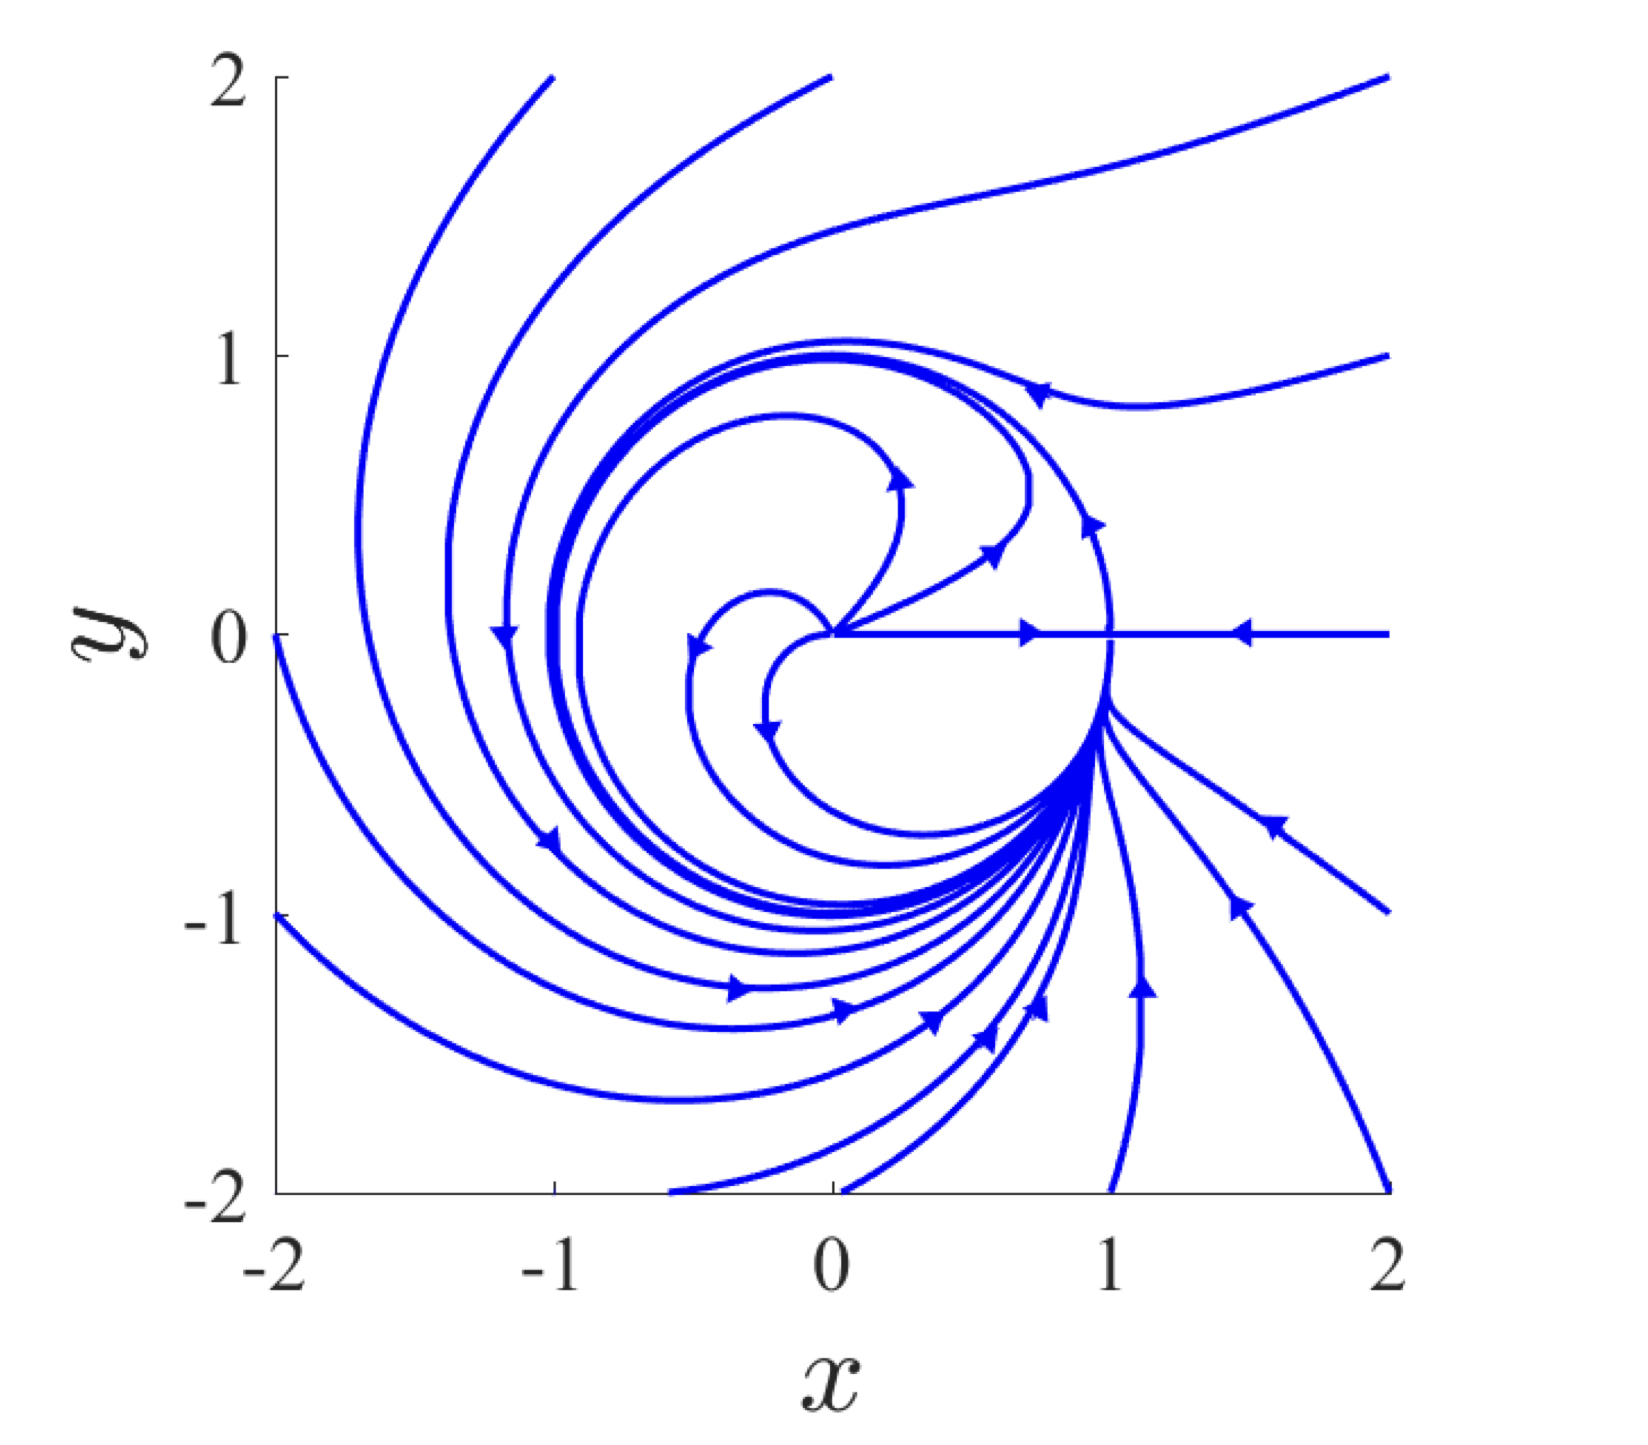
\includegraphics[scale=0.2]{./images/phase_portrait3.jpeg}
  	\centering
    \caption{The attractive equilibrium (1,0) is not stable}\label{phase_portrait3}
\end{figure}

\newmdtheoremenv[style=defEnv]{homoclinic and heteroclinic orbits}[theorem]{Definition}
\begin{homoclinic and heteroclinic orbits}
    Consider the differential equation~\eqref{eq:autonomousDE} with associated flow
    $\varphi$.
    \begin{enumerate}[label = (\roman*)]
        \item An orbit $O(x)$ for some $x\in D$ is called a \textbf{homoclinic
            orbit} if there exists an equilibrium $x^*\in D\backslash\{x\}$ s.t.
            \[
                \lim_{t\rightarrow\infty}\varphi(t,x)=x^*,
                \quad \lim_{t\rightarrow-\infty}\varphi(t,x)=x^*.
            \]
        \item An orbit $O(x)$ for some $x\in D$ is called a \textbf{heteroclinic
            orbit} if there exists two different equilibria $x_1^{*}\neq
            x_2^{*}\in D$ s.t.
            \[
                \lim_{t\rightarrow\infty}\varphi(t,x)=x_1^{*},
                \quad \lim_{t\rightarrow-\infty}\varphi(t,x)=x_2^{*}.
            \]
    \end{enumerate} 
\end{homoclinic and heteroclinic orbits}

\subsection{Stability of linear systems}

\newmdtheoremenv[style=defEnv]{stability of linear systems}[theorem]{Theorem}
\begin{stability of linear systems}
    Consider the autonomous linear system
    \[
        \dot{x}=Ax,
    \]
    where $A\in\mathbb{R}^{d\times d}$. Then the trivial equilibrium $x^*=0$ of
    this system is
    \begin{enumerate}[label = (\roman*)]
        \item stable iif the following two statements hold:
            \begin{enumerate}[label = (\alph*)]
                \item the real part of all eigenvalues of $A$ is non-positive,
                    i.e.\ we have $\text{Re}\,\rho\le 0$ for all eigenvalues
                    $\rho$ of $A$, and
                \item the eigenvalue $\rho$ is semi-simple for all eigenvalues
                    $\rho$ of $A$ with $\text{Re}\,\rho=0$.
            \end{enumerate} 
        \item exponentially stable iif $\text{Re}\,\rho<0$ for all eigenvalues 
            $\rho$ of $A$.
    \end{enumerate} 
\end{stability of linear systems}

\subsection{Hyperbolicity}

\newmdtheoremenv[style=defEnv]{hyperbolicity}[theorem]{Definition}
\begin{hyperbolicity}
    A matrix $A\in\mathbb{R}^{d\times d}$ is called \textbf{hyperbolic}
    if all eigenvalues $\lambda$ of $A$ have non-zero part, i.e.\
    $\text{Re}\,\lambda\neq 0$. An equilibrium $x^*$ of a differential equation
    \[
        \dot{x}=f(x),
    \]
    where $f:D\subset \mathbb{R}^{d}\rightarrow\mathbb{R}^{d}$ is continuously
    differentiable, is called \textbf{hyperbolic} if the matrix
    $f'(x^*)\in\mathbb{R}^{d\times d}$ is hyperbolic.
\end{hyperbolicity}

\newtheorem{1d non-hyperbolicity}[theorem]{Example}
\begin{1d non-hyperbolicity}
    We consider the linear one-dimensional differential equation
    \[
        \dot{x}=0.
    \]
    Then the trivial equilibrium $x^* =0$ is stable, and the derivative $f'(x^*)$
    of the RHS ($f(x)=0\;\forall x\in\mathbb{R}$) is 0,
    and thus this equilibrium (and all other equilibria0 is non-hyperbolic.
    We consider the following nonlinear perturbations and discuss its effect on
    the stability of $x^*=0$:
    \begin{enumerate}[label = (\roman*)]
        \item $\dot{x}=x^2$: the equilibrium $x^*=0$ becomes unstable,
            although it attracts all points starting in the negative half-line.
        \item $\dot{x}=-x^2$: the equilibrium $x^*=0$ becomes unstable,
            although it attracts all points starting in the negative half-line.
        \item $\dot{x}=x^{3}$: the equilibrium $x^*=0$ becomes unstable, and all
            points (except $x^*$) move away from $x^*$ forward in time.
        \item $\dot{x}=-x^{3}$: the equilibrium $x^*=0$ becomes asymptotically
            stable, but it is not exponentially stable.
    \end{enumerate} 
\end{1d non-hyperbolicity}

\subsection{Linearised stability}

\newmdtheoremenv[style=defEnv]{gronwall lemma}[theorem]{(Gronwall lemma) Lemma}
\begin{gronwall lemma}
    We consider a continuous function $u:[a,b]\rightarrow\mathbb{R}$ defined on
    an interval $[a,b]$, and let $c,d\ge 0$. We assume that the function $u$
    satisfies the implicit inequlity
    \[
        0\le u(t)\le c + d \int_{a}^{t} u(s)\mathrm{d}s\quad\forall t\in[a,b].
    \]
    Then we have the explicit estimate
    \[
        u(t)\le ce^{d(t-a)}\quad\forall t\in[a,b].
    \]
\end{gronwall lemma}

\newmdtheoremenv[style=defEnv]{linearised stability}[theorem]{Theorem}
\begin{linearised stability}\label{linearised stability}
    Let $D\subset \mathbb{R}^{d}$ be open and $f:D\rightarrow\mathbb{R}^{d}$
    be continuously differentiable, and consider the autonomous differential
    equation
    \[
        \dot{x}=f(x).
    \]
    Assume that $x^*$ is an equilibrium of the above equation (i.e.\ $f(x^*)=0$)
    s.t. for all eigenvalues $\lambda\in\mathbb{C}$ of the linearisation 
    $f'(x^*)\in\mathbb{R}^{d\times d}$, we have $\text{Re}\,\lambda<0$.
    Then the equilibrium $x^*$ is exponentially stable.
\end{linearised stability}

\newtheorem{pendulum, exponentially stable equilibrium}[theorem]{Example}
\begin{pendulum, exponentially stable equilibrium}
    Consider a pendulum moving along a circle of radius $r>0$, with a mass $m>0$
    and friction coefficient $k>0$. Let $x$ denote the angle from the vertical.
    The force tangential ot the circle depends on both the position $x$ and the
    speed $\dot{x}$ of the pendulum, and is given by
    \[
        F_{\text{tan}}(x,\dot{x})=-mg\sin(x)-kr\dot{x}.
    \]
    Newton's law reads as $mr\ddots{x}=F_{\text{tan}}(x,\dot{x})$, and thus we
    get the second-order one-dimensional differential equation
    \[
        \ddot{x}=-\frac{g}{r}\sin(x)-\frac{k}{m}\dot{x},
    \]
    which can be transformed into the first-order two-dimensional system
    \begin{align*}
        \dot{x} & = y,
        \dot{y} = -\frac{g}{r}\sin(x)-\frac{k}{m}y.
    \end{align*} 
    The matrix of the linearisation at (0, 0) is
    \[
        \begin{pmatrix}
            \frac{\mathrm{d}\dot{x}}{\mathrm{d}x} & \frac{\mathrm{d}\dot{x}}{\mathrm{d}y} \\
            \frac{\mathrm{d}\dot{x}}{\mathrm{d}y} & \frac{\mathrm{d}\dot{y}}{\mathrm{d}y} \\
        \end{pmatrix} =
        \begin{pmatrix}
            0 & 1 \\
            -\frac{g}{r} & -\frac{k}{m}
        \end{pmatrix} 
    \]
    which gives two eigenvalues
    $\lambda_{\pm}:=\frac{1}{2}\left(-\frac{k}{m}\pm\sqrt{{\left(\frac{k}{m}\right)}^{2}-\frac{4g}{r}}\right)$.
    It follows that the real parts of both eigenvalues $\lambda_{\pm}$ are
    negative, and hence, Theorem~\ref{linearised stability} implies that the
    equilibria $(n\pi,0)$ for $n$ even are exponentially stable.
\end{pendulum, exponentially stable equilibrium}

\subsection{Stable and unstable sets, invariant sets}

\newmdtheoremenv[style=defEnv]{stable and unstable set}[theorem]{Definition}
\begin{stable and unstable set}
    Consider the differential equation~\eqref{eq:autonomousDE} with associated flow
    $\varphi$, and let $x^*$ be an equilibrium.
    We define the \textbf{stable set} of $x^*$ as
    \[
        W^{s}(x^{*}):=\left\{x\in D:\lim_{t\rightarrow\infty}\varphi(t,x)=x^{*}\right\},
    \]
    and the \textbf{unstable set} of $x^*$ is defined as
    \[
        W^{u}(x^*)a:=\left\{x\in D:\lim_{t\rightarrow-\infty}\varphi(t,x)=x^*\right\}.
    \]
    Note that if $x^*$ is an attractive equilibrium, then $W^{s}(x^*)$ is
    called \textbf{domain of attraction}, and it follows from the definition of
    attractivity that this is sa neighbourhood of $x^*$. Moreover,
    $W^{s}(x^*)$ is an open set in this case.
\end{stable and unstable set}

\newmdtheoremenv[style=defEnv]{invariance}[theorem]{Definition}
\begin{invariance}
    Consider the differential equation~\eqref{eq:autonomousDE}.
    Then a set $M\subset D$ is called
    \begin{enumerate}[label = (\roman*)]
        \item \textbf{positively invariant} if $\forall x\in M$,
            we have $O^{+}(x)\subset M$.
        \item \textbf{negatively invariant} if $\forall x\in M$,
            we have $O^{-}(x)\subset M$.
        \item \textbf{invariant} if $\forall x\in M$,
            we have $O(x)\subset M$.
    \end{enumerate} 
\end{invariance}
Note that sets that consist of equilibria or periodic orbits are invariant.
Stable and unstable sets are also invariant positively and negatively,
and any union of orbits is invariant.
Accordingly unions of half-orbits of the form $O^{+}(x)$ or $O^{-}(x)$
are positively invariant or negatively invariant, respectively.

\section{Limit sets}

We study an autonomous differential equation of the form
\begin{equation}\label{eq:limitDE}
    \dot{x}=f(x),
\end{equation} 
where $f:D\rightarrow\mathbb{R}^{d}$ is locally Lipschitz continuous and
$D\subset\mathbb{R}^{d}$ is an open set.
We denote the flow of this differential equation by $\varphi$.

\newmdtheoremenv[style=defEnv]{Omega and alpha limit sets}[theorem]{Definition}
\begin{Omega and alpha limit sets}
    Consider the flow $\varphi$ of the differential equation~\eqref{eq:limitDE},
    and let $x\in D$.
    \begin{enumerate}[label = (\roman*)]
        \item A point $x_\omega\in D$ is called \textbf{omega limit point} of
            $x$, if there exists a sequence ${\{t_n\}}_{n\in\mathbb{N}}$
            s.t. $\lim_{n\rightarrow\infty}t_n=\infty$ and
            \[
                x_\omega=\lim_{n\rightarrow\infty}\varphi(t_n,x).
            \]
            We denote by $\omega(x)$ the set of all omega limit points of $x$.
            $\omega(x)$ is called \textbf{omega limit set} of $x$.
        \item A point $x_\alpha\in D$ is called \textbf{alpha limit point} of
            $x$, if there exists a sequence ${\{t_n\}}_{n\in\mathbb{N}}$
            s.t. $\lim_{n\rightarrow\infty}t_n = -\infty$ and
            \[
                x_\alpha = \lim_{n\rightarrow\infty}\varphi(t_n, x).
            \]
            We denote by $\alpha(x)$ the set of all alpha limit points of $x$.
            $\alpha(x)$ is called \textbf{alpha limit set} of $x$.
    \end{enumerate} 
\end{Omega and alpha limit sets}
Note that the omega limit set of a point $x$ is empty if
$\sup{J_{\text{max}}(x)}<\infty$, and the alpha limit set to be nonempty
requires $\inf{J_{\text{max}}(x)}=-\infty$.

\newmdtheoremenv[style=defEnv]{alternative characterisation of limit sets}[theorem]{Proposition}
\begin{alternative characterisation of limit sets}
    Consider the flow $\varphi$ of the differential equation~\eqref{eq:limitDE},
    and let $x\in D$. Then we have
    \[
        \omega(x)=\bigcap_{t\ge 0}\overline{O^{+}(\varphi(t,x))},
        \alpha(x)=\bigcap_{t\le 0}\overline{O^{-}(\varphi(t,x))}.
    \]
\end{alternative characterisation of limit sets}

\newmdtheoremenv[style=defEnv]{properties of omega and alpha limit sets}[theorem]{Proposition}
\begin{properties of omega and alpha limit sets}
    Consider the differential equation~\eqref{eq:limitDE}, and let $x\in D$.
    Then the following statements hold.
    \begin{enumerate}[label = (\roman*)]
        \item The omega limit set $\omega(x)$ is invariant.
            In addition, if $O^{+}(x)$ is bounded and 
            $\overline{O^+(x)}\subset D$, 
            then $\omega(x)$ is non-empty and compact.
        \item The alpha limit set $\alpha(x)$ is invariant.
            In addition, if $O^{-}(x)$ is bounded and 
            $\overline{O^-(x)}\subset D$, 
            then $\alpha(x)$ is non-empty and compact.
    \end{enumerate} 
\end{properties of omega and alpha limit sets}

\section{Lyapunov functions}

\newmdtheoremenv[style=defEnv]{orbital derivative}[theorem]{Definition}
\begin{orbital derivative}
    Consider the differential equation~\eqref{eq:limitDE}, and let
    $V:D\rightarrow\mathbb{R}$ be a continuously differentiable function.
    Then the \textbf{orbital derivative} $\dot{V}$ of the function $V$ is defined by
    \[
        \dot{V}(x):=V'(x)\cdot f(x)
        =\sum_{i=1}^{d} \frac{\partial V}{\partial x_i}(x)f_i(x),
    \]
    which describes the derivative of $V$ along solutions $\mu:I\rightarrow D$
    of~\eqref{eq:limitDE}. This follows from
    \[
        \frac{\mathrm{d}}{\mathrm{d}t}V(\mu(t))=V'(\mu(t))\cdot\dot{\mu}(t)
        = \dot{V}(\mu(t))\quad\forall t\in I.
    \]
\end{orbital derivative}

\newmdtheoremenv[style=defEnv]{Lyapunov function}[theorem]{Definition}
\begin{Lyapunov function}
    Consider the differential equation~\eqref{eq:limitDE}, and let 
    $V:D\rightarrow\mathbb{R}$ be a continuously differentiable function.
    Then $V$ is called a \textbf{Lyapunov function} if
    \[
        \dot{V}(x)\le 0\quad\forall x \in D,
    \]
    which decreases along solutions, i.e.\
    \[
        V(\varphi(t,x))\le V(x)\quad\forall t\in[0,\sup{J_{\text{max}}(x)}).
    \]
\end{Lyapunov function}

\newmdtheoremenv[style=defEnv]{sublevel sets of Lyapunov functions are +ve invariant}[theorem]{Proposition}
\begin{sublevel sets of Lyapunov functions are +ve invariant}
    Consider the differential equation~\eqref{eq:limitDE} with a Lyapunov
    function $V:D\rightarrow\mathbb{R}$. Then any sublevel set of the form
    \[
        S_c:=\left\{x\in D:V(x)\le c\right\},
    \]
    where $c\in\mathbb{R}$, is positively invariant.
\end{sublevel sets of Lyapunov functions are +ve invariant}

\newmdtheoremenv[style=defEnv]{Lyapunov's direct method for stability}[theorem]{Theorem}
\begin{Lyapunov's direct method for stability}
    Consider the differential equation~\eqref{eq:limitDE} with an equilibrium 
    $x^*\in D$, and let $V:D\rightarrow\mathbb{R}$ be a Lyapunov function s.t.
    \[
        V(x^*)=0 \quad\text{and}\quad V(x)>0\quad\forall x\in D\backslash\{x^*\}.
    \]
    Then the equilibrium $x^*$ is stable.
\end{Lyapunov's direct method for stability}

\newtheorem{application of Lyapunov's direct method for stability}[theorem]{Example}
\begin{application of Lyapunov's direct method for stability}
    We consider the two-dimensional differential equation
    \begin{align*}
        \dot{x} & = -y-xy^{2} \\
        \dot{y} & = x-yx^{2}.
    \end{align*} 
    The only equilibrium of this system is the trivial equilibrium (0, 0).
    The linearisation in (0, 0) is given by $\begin{pmatrix}
        0 & -1\\
        1 & 0
    \end{pmatrix} $, and thus the system is non-hyperbolic and stability cannot
    be deduced from Theorem~\ref{linearised stability}.

    We first show that the trivial equilibrium is stable by considering the
    quadratic function $V(x,y)=x^{2}+y^2$ for all $(x,y)\in\mathbb{R}^{2}$. Then
    \[
        \dot{V}(x,y)=V'(x,y)\cdot f(x,y)=(2x,2y)\begin{pmatrix}
                -y-xy^{2} \\
                x-yx^{2}
        \end{pmatrix} = -4x^{2}y^{2}\le 0,
    \]
    so (0, 0) is stable. 
\end{application of Lyapunov's direct method for stability}

\newmdtheoremenv[style=defEnv]{La salle's invariance principle}[theorem]{Theorem}
\begin{La salle's invariance principle}
    Consider the differential equation~\eqref{eq:limitDE} with a Lyapunov
    function $V:D\rightarrow\mathbb{R}$. Then
    \[
        \omega(x)\subset\left\{y\in D:\dot{V}(y)=0\right\}
        \quad\forall x\in D.
    \]
\end{La salle's invariance principle}

\newmdtheoremenv[style=defEnv]{reformulation of La salle's invariance principle}[theorem]{Corollary}
\begin{reformulation of La salle's invariance principle}
    Consider the differential equation~\eqref{eq:limitDE} with a Lyapunov
    function $V:D\rightarrow\mathbb{R}$. Then for any $x\in D$, 
    $\omega(x)$ is contained in the largest invariant subset of 
    $\left\{y\in D:\dot{V}(y)=0\right\}$. Here the largest invariant subset is
    given by the union of invariant subsets of $\left\{y\in
    D:\dot{V}(y)=0\right\}$.
\end{reformulation of La salle's invariance principle}

\newmdtheoremenv[style=defEnv]{Lyapunov's direct method for asymptotic stability}[theorem]{Theorem}
\begin{Lyapunov's direct method for asymptotic stability}\label{test asymptotic stability}
    Consider the differential equation~\eqref{eq:limitDE} with an equilibrium
    $x^*\in D$, and let $V:D\rightarrow\mathbb{R}$ be a Lyapunov function s.t.
    \begin{align*}
        V(x^*)=0 && \text{and} && V(x)>0 \quad\forall x\in D\backslash\{x^*\}, \\
        \dot{V}(x^*)=0 && \text{and} && \dot{V}(x)<0 \quad\forall x\in D\backslash\{x^*\}.
    \end{align*} 
    Then the equilibrium $x^*$ is asymptotically stable.
\end{Lyapunov's direct method for asymptotic stability}

\newmdtheoremenv[style=defEnv]{sublevell sets of Lyapunov functions are ...}[theorem]{Corollary}
\begin{sublevell sets of Lyapunov functions are ...}
    Under the assumptions of Theorem~\ref{test asymptotic stability}, we
    consider the sublevel sets of the Lyapunov function $V$, which are of the
    form
    \[
        S_c:=\left\{x\in D:V(x)\le c\right\},
    \]
    where $c>0$. Then $S_c$ is a subset of the domain of attraction
    $W^{s}(x^{*})$ if $S_c\subset D$ is compact.
\end{sublevell sets of Lyapunov functions are ...}

\section{Poincar\'{e}-Bendixson theorem}

\newmdtheoremenv[style=defEnv]{Poincare-Bendixson
theorem}[theorem]{(Poincar\'{e}-Bendixson theorem) Theorem}
\begin{Poincare-Bendixson theorem}
    Consider the differential equation~\eqref{eq:limitDE},
    and assume that for some $x\in D$, $O^{+}(x)$ lies in a compact subset $K$
    of $D$, which contains not more than finitely many equilibria.
    Then one of the following three statements holds for $\omega(x)$.
    \begin{enumerate}[label = (\roman*)]
        \item $\omega(x)$ is a singleton consisting of an equilibrium.
        \item $\omega(x)$ is a periodic orbit.
        \item $\omega(x)$ consists of equilibria and non-closed orbits.
            The non-closed orbits in $\omega(x)$ converge forward and backward
            in time to equilibria in $\omega(x)$, so they are either homoclinic
            or heteroclinic orbits.
    \end{enumerate} 
\end{Poincare-Bendixson theorem}

\newmdtheoremenv[style=defEnv]{existence of a periodic orbit}[theorem]{Corollary}
\begin{existence of a periodic orbit}
    Consider the differential equation~\eqref{eq:limitDE},
    and assume that for some $x\in D$, $O^+(x)$ lies in a compact subset $K$ of
    $D$ that does not contain an equilibrium. 
    Then $\omega(x)$ is a periodic orbit.
\end{existence of a periodic orbit}

\newtheorem{existence of orbit}[theorem]{Example}
\begin{existence of orbit}
    We consider the two-dimensional differential equation
    \begin{align*}
        \dot{x} & = y, \\
        \dot{y} & = -x+y(1-x^{2}-2y^{2}).
    \end{align*} 
    We first show that $M:=\left\{(x,y)\in\mathbb{R}^{2}:\frac{1}{3}\le
    x^{2}+y^{2}\le 2\right\}$ is positively invariant.
    We show that the vector field of the RHS points inwards at the boundary of
    $M$. More precisely, we consider the scalar-valued function
    $V(x,y)=x^{2}+y^{2}$ and show that the orbital derivative $\dot{V}$
    satisfies $\dot{V}(x,y)<0$ for $x^{2}+y^{2}=2$ and $\dot{V}(x,y)>0$ for
    $x^{2}+y^{2}=\frac{1}{3}$.
    Firstly, the orbital derivative reads as
    \[
        \dot{V}(x,y)=(2x, 2y)\begin{pmatrix}
                y\\
                -x+y(1-x^{2}-2y^{2})
            \end{pmatrix} =2y^{2}(1-x^{2}-2y^{2}).
    \]
    For $x^{2}+y^{2}=2$, we have $\dot{V}(x,y)=2y^{2}(-1-y^{2})<0$
    and for $x^{2}+y^{2}=\frac{1}{3}$, we have
    $\dot{V}(x,y)=2y^{2}(\frac{2}{3}-y^{2})\ge 0$.
    This shows the positive invariance of $M$.
    Note that the only equilibrium is clearly given by $(0,0)\notin M$.
    We apply the corollary to the Poincar\'{e}-Bendixson theorem (previous
    corollary) and conclude that the positively invariant set $M$ contains a
    periodic orbit.
\end{existence of orbit}



\end{document}
